\chapter{Anything From Anywhere!}
\section{Mathematics}
\begin{note}[Linear Interpolation]

In mathematics, linear interpolation is a method of curve fitting using linear polynomials to construct new data points within the range of a discrete set of known data points.It's simply a line between two given points.
\begin{center}
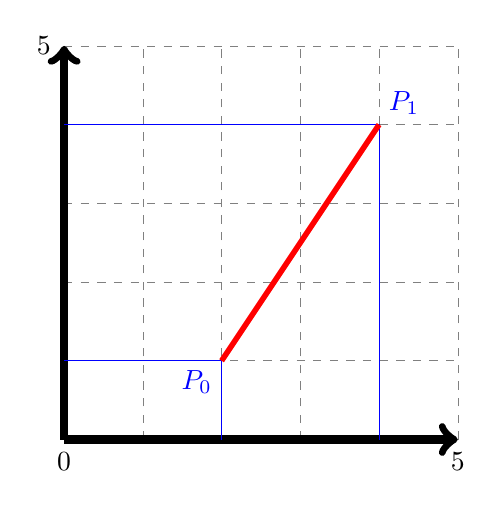
\begin{tikzpicture}
\draw[help lines, style=dashed] (0,0) grid (5,5);
\draw[->, line width = 3pt] (0,0) [below] node {0} -- (0,5) [left] node {5} ;
\draw[->, line width = 3pt] (0,0) -- (5,0) [below] node {5};
\draw[blue] (0,1) -- (2,1) [below left] node {$P_0$} -- (2,0);
\draw[blue] (0,4) -- (4,4) [above right] node {$P_1$} -- (4,0);
\draw[red, line width = 2pt] (2,1) -- (4,4);
\end{tikzpicture}
\end{center}
Given the two points of $P_0 (2,1)$ and $P_1 (4,4)$, the red line is the linear interpolant between the points. The linear interpolant  $L$ between two general points $P_0 = (x_0,y_0)$ and $P_1 (x_1,y_1)$ is computed by the equations \ref{eqnLinearInter1} or \ref{eqnLinearInter2}.
\begin{equation} \label{eqnLinearInter1}
\frac{y-y_0}{x-x_0} = \frac{y_1-y_0}{x_1-x_0} 
\end{equation}
\begin{equation} \label{eqnLinearInter2}
\mathbf {L} (t)=\mathbf {P} _{0}+t(\mathbf {P} _{1}-\mathbf {P} _{0})=(1-t)\mathbf {P} _{0}+t\mathbf {P} _{1}{\mbox{ , }}0\leq t\leq 1
\end{equation}
\end{note}

\begin{note}[Bézier curve]

A Bézier curve is a parametric curve frequently used in computer graphics and related fields. In vector graphics, Bézier curves are used to model smooth curves that can be scaled indefinitely. ``Paths", as they are commonly referred to in image manipulation programs, are combinations of linked Bézier curves.

A Bézier curve is defined by a set of control points $P_0$ through $P_n$, where $n$ is called its order (n = 1 for linear, 2 for quadratic, etc.). The first and last control points are always the end points of the curve; however, the intermediate control points (if any) generally do not lie on the curve.
\begin{itemize}
\item Linear Bézier curves:
Given points P0 and P1, a linear Bézier curve is simply a straight line between those two points. The curve is given by\\
\begin{equation}
\mathbf {B} (t)=\mathbf {P} _{0}+t(\mathbf {P} _{1}-\mathbf {P} _{0})=(1-t)\mathbf {P} _{0}+t\mathbf {P} _{1}{\mbox{ , }}0\leq t\leq 1
\end{equation}
and is equivalent to linear interpolation.
\item Quadratic Bézier curves:
A quadratic Bézier curve is the path traced by the function B(t), given points P0, P1, and P2,
\begin{equation}
\mathbf {B} (t)=(1-t)[(1-t)\mathbf {P} _{0}+t\mathbf {P} _{1}]+t[(1-t)\mathbf {P} _{1}+t\mathbf {P} _{2}]{\mbox{ , }}0\leq t\leq 1
\end{equation} ,which can be interpreted as the linear interpolant of corresponding points on the linear Bézier curves from P0 to P1 and from P1 to P2 respectively. Rearranging the preceding equation yields:
\begin{equation}
\mathbf {B} (t)=(1-t)^{2}\mathbf {P} _{0}+2(1-t)t\mathbf {P} _{1}+t^{2}\mathbf {P} _{2}{\mbox{ , }}0\leq t\leq 1.
\end{equation}
The derivative of the Bézier curve with respect to t is
\begin{equation}
\mathbf {B} '(t)=2(1-t)(\mathbf {P} _{1}-\mathbf {P} _{0})+2t(\mathbf {P} _{2}-\mathbf {P} _{1})\,.
\end{equation} 
from which it can be concluded that the tangents to the curve at P0 and P2 intersect at P1. As t increases from 0 to 1, the curve departs from P0 in the direction of P1, then bends to arrive at P2 from the direction of P1.
The second derivative of the Bézier curve with respect to t is
\begin{equation}
\mathbf {B} ''(t)=2(\mathbf {P} _{2}-2\mathbf {P} _{1}+\mathbf {P} _{0})
\end{equation}

\begin{center}
\includegraphics[scale=0.8]{Images/etc/bei}
\end{center}


\end{itemize}


\end{note}